This where I fell down in the initial lab where I didn't fully verify my outputs against a known good output. To compensate for that I can now properly verify the implemented CRC init register by checking various different init values and comparing them to the online calculator. 

\centering{Checking 0xF0F0}
\begin{figure}[H]
    \centering
    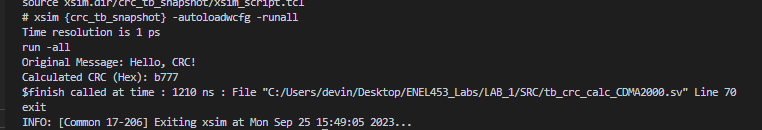
\includegraphics[width = 10cm]{Lab_1/Lab_1_Correction/Images/0F0F_verification.png}
    \caption{Simulation Results}
    \label{fig:simulationresult}
\end{figure}
\begin{figure}[H]
    \centering
    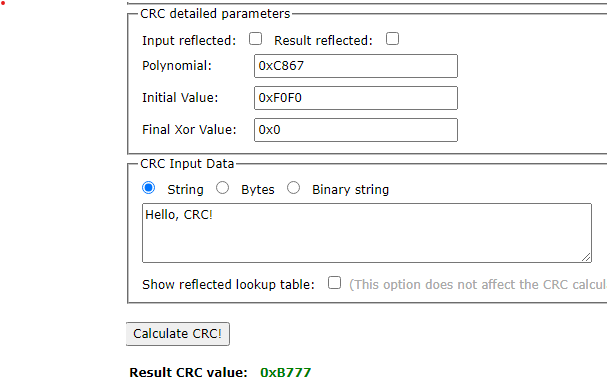
\includegraphics[width = 10cm]{Lab_1/Lab_1_Correction/Images/0F0F_verificationsite.png}
    \caption{Online Calculator}
    \label{fig:online_calc}
\end{figure}

I then asked a random number generator to generate me 3 more possible tests. It decided on EE73, 5A48, and E781. 

\begin{verbatim}
    Original Message: Hello, CRC!
    Calculated CRC (Hex): bf45
\end{verbatim}

\begin{verbatim}
    Result CRC value: 0xBF45
\end{verbatim}

\begin{verbatim}
    Original Message: Hello, CRC!
    Calculated CRC (Hex): dda1
\end{verbatim}

\begin{verbatim}
    Result CRC value: 0xDDA1
\end{verbatim}

\begin{verbatim}
    Original Message: Hello, CRC!
    Calculated CRC (Hex): d0d5
\end{verbatim}

\begin{verbatim}
    Result CRC value: 0xD0D5
\end{verbatim}

\RaggedRight
Given the outputs for each of these confirms with the tools this would suggest that it is very likely that the implementation is now fully correct. If moving this to silicon however, we would likely want to mirror our implementation in another more friendly language and verify across a number of randomized test inputs that the results match.